\title{Masters thesis}
\author{Aleksander Mendoza}

\documentclass[12pt]{article}
\usepackage{tikz}
\usepackage[utf8]{inputenc}
\usepackage[T1]{fontenc}
\usepackage{lmodern}
\usepackage{amsfonts}
\usepackage{mathrsfs}
\usepackage{centernot}
\usepackage{listings}
\usepackage{mathtools}
\usepackage{xcolor}
\usepackage{amsthm}
\usepackage{amsmath}
\usepackage{amssymb}
\usepackage{tikzit}
\usepackage{siunitx}
\usepackage[hidelinks]{hyperref}
\usepackage{tabularx}
\usepackage{enumitem}
\usepackage{chemformula}
\input{style.tikzstyles}
\def\MakeUppercaseUnsupportedInPdfStrings{\scshape}
\DeclareMathOperator*{\argmax}{argmax}
\DeclareMathOperator*{\argmin}{argmin}
\DeclareMathOperator*{\hot}{hot}
\newtheorem{definition}{Definition}
\newtheorem{theorem}{Theorem}[section]
\newtheorem{corollary}{Corollary}[theorem]
\newtheorem{lemma}[theorem]{Lemma}
\renewcommand{\labelenumii}{\theenumii}
\renewcommand{\theenumii}{\theenumi.\arabic{enumii}.}
\DeclareSIUnit{\molar}{M}
\begin{document}
\maketitle
\lstset{
	basicstyle=\ttfamily,
	mathescape
}


\begin{abstract}
	abstract here
\end{abstract} 
\tableofcontents
\section{Introduction}

Modern deep neural networks have achieved many impressive feats, yet at the same time their intelligence appears to be shallow and inflexible. Perhaps the most challenging is the frontier of reinforcement learning.  As it has been demonstrated in Deepmind's ablation studies \cite{rainbow_dqn}, deep RL requires absurd amounts of training data and computation power (figure \ref{fig:dqn}). This issue is often referred to as sample inefficiency.
\begin{figure}[!htbp]
	\centering
	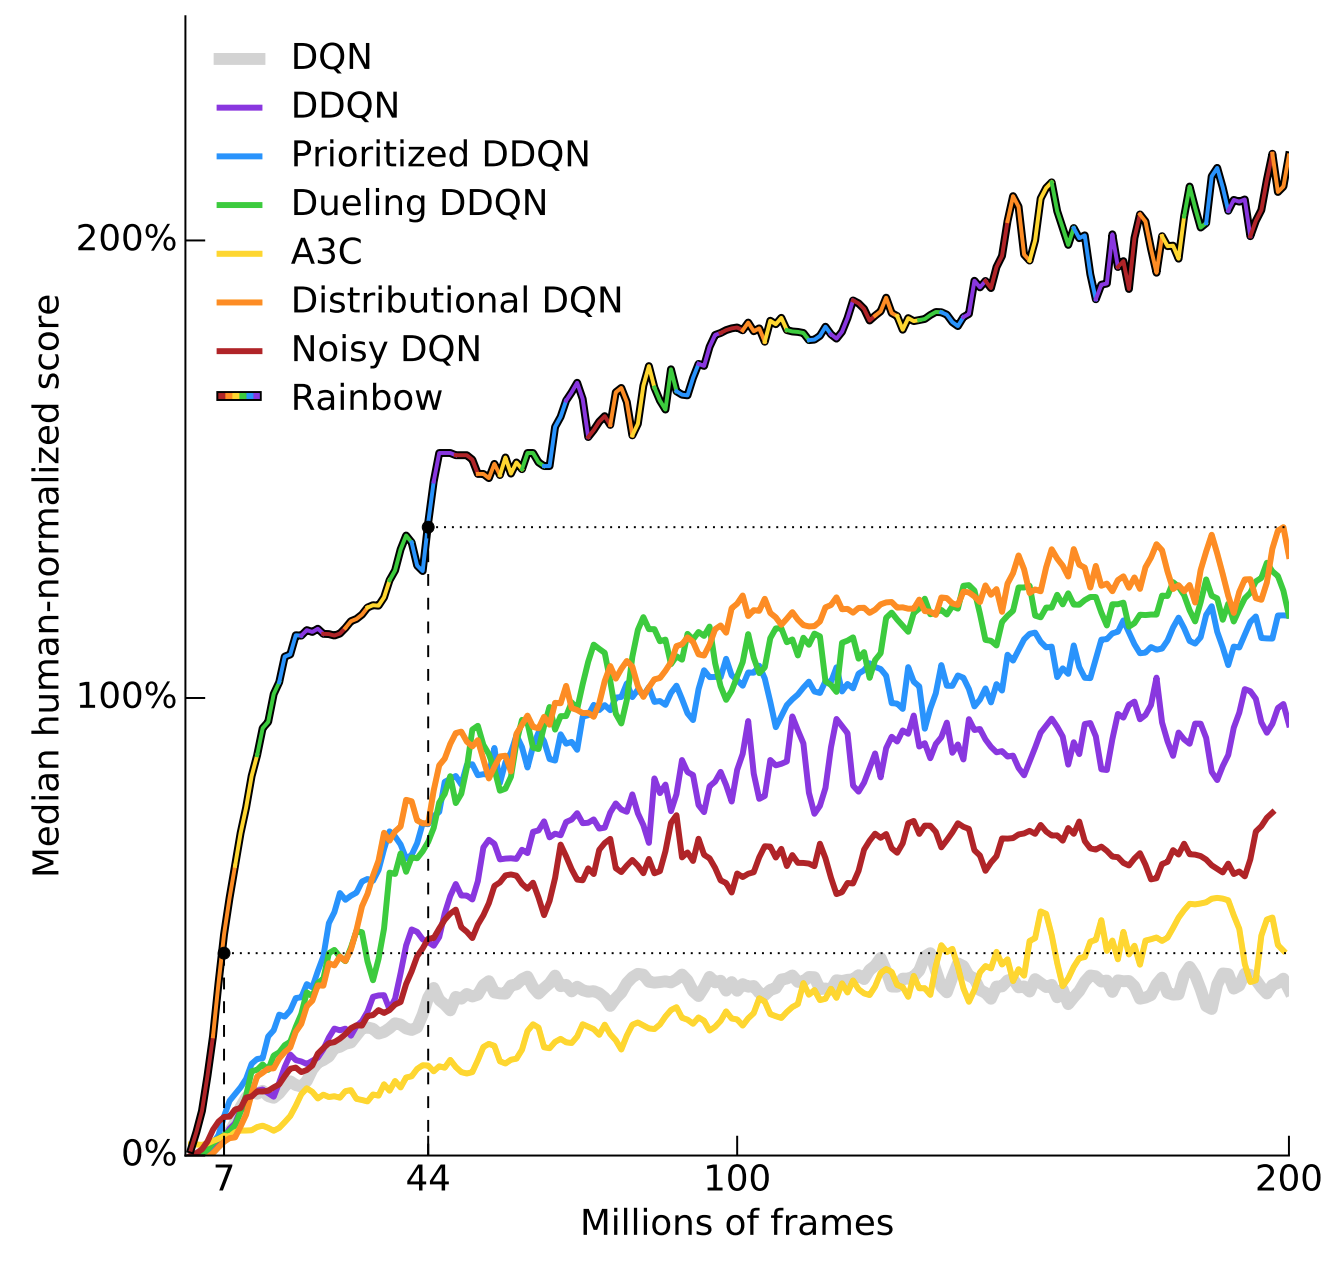
\includegraphics[width=13cm]{dqn}
	\caption{Median human-normalized performance across
		57 Atari games for various deep RL methods.}
	\label{fig:dqn}
\end{figure} 
The produced results rarely generalise to novel tasks and often fail to adapt to slight variations of the same task \cite{generalisation_in_rl}. Transfer learning does not exist in deep RL and fine-tuning an agent on a novel task leads to ``catastrophic forgetting'' of the previous one. Moreover, even within the same environment, reproducibility suffers and learning algorithms may fail due to random fluctuations\cite{vime} as it can be seen on figure \ref{fig:vime}. 
\begin{figure}[!htbp]
	\centering
	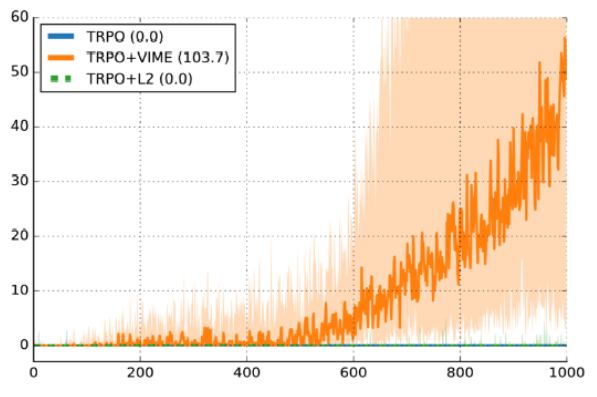
\includegraphics[width=13cm]{vime}
	\caption{The dark line is the median performance over 10 random seeds. Shaded region is the 25th to 75th percentile. It means that 25\% of runs fail due to randomness.}
	\label{fig:vime}
\end{figure} 
Biological brains do not suffer from these problems. In this thesis, I attempt to investigate what nature can tell us about reinforcement learning. How could we solve the problems of sample inefficiency and catastrophic forgetting? Is deep learning the right approach?

\subsection{Neuronal dynamics}

\subsubsection{Hodgkin-Huxley model}

In order to understand how nature tackles the problems of reinforcement learning, first we should understand some fundamentals of neuroscience. 

Like many natural phenomena, biological brains can be modelled on many different levels of complexity. The smallest possible scale is miscroscopic - the biophysics of individual neurons. In 1952, Hodgkin and Huxley \cite{hodgkin} have successfully described the evolution of membrane potentials using differential equations. Their model was able to perfectly fit the observed data (figure \ref{fig:hodgkin_huxley_experiments}). 
\begin{figure}[!htbp]
	\centering
	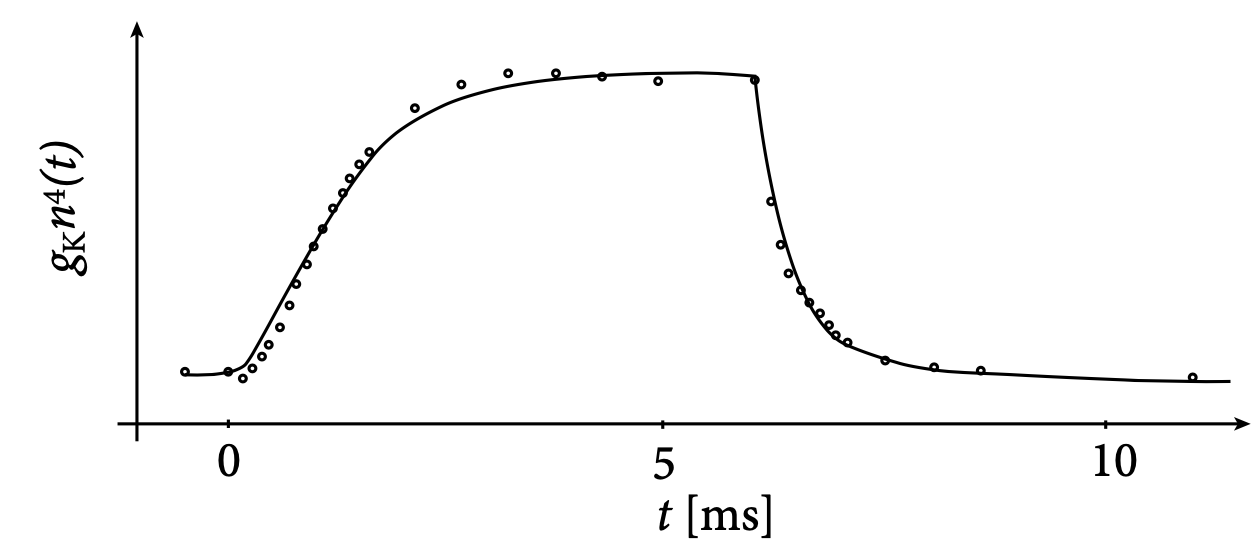
\includegraphics[width=13cm]{hodgkin_huxley_experiments}
	\caption{Experimental measurements (dots) and predictions of Hodgkin-Huxley model  (line) }
	\label{fig:hodgkin_huxley_experiments}
\end{figure} 

They reduced the neuron into a simple electric circuit. The fluid inside a cell body is insulated from the outside environment by a membrane, which cats as a capacitor $C$. It can store certain charge $q$ in form of ions such as $\ch{K+}$, $\ch{Na+}$, $\ch{Cl-}$. Let $n(x_1)$ and $n(x_2)$ denote the concentration of ions inside and outside the cell body respectively. 
The difference in concentration leads to difference in electric potential 
$\Delta u = u(x_1) - u(x_2)$. 
From thermodynamics we know that 
$n(x)\propto \exp(\frac{-E(x)}{kT})$, 
where $E(x)$ is the energy a location $x$, $T$ is temperature and $k$ is the Boltzmann constant. Electric energy is given by $E(x)=qu(x)$, therefore we obtain
\[
\frac{n(x_1)}{n(x_2)} = \exp\big(-\frac{qu(x_1)-qu(x_2)}{kT}\big)
\]
From this we can derive Nernst equation 
\[
\Delta u = \frac{kT}{q}\ln\frac{n(x_1)}{n(x_2)}
\]
For example, it has been estimated that concentration of $\ch{K+}$ is $\approx\SI{140}{\milli\molar}$ inside the cell  and  $\approx\SI{5}{\milli\molar}$ outside. Potassium has charge $q=\SI{1.6e-19}{\coulomb}$. Applying it to the formula with $k=\SI{1.4e-23}{\joule/\kelvin}$ yields Nernst potential of $E_{\ch{K}}=\SI{-83}{\milli\volt}$ at equilibrium. If the membrane potential $\Delta u$ falls below $E_{\ch{K}}$ (for example when experimenter injects current from outside)

By maintaining  certain ionic concentration $n(x_1)$, neurons can store voltage like batteries. The cell membrane is a nearly perfect insulator but on it's surface there many ion gates, which allow certain particles to pass through. Hodgkin and Huxley model those as resistance $R$. If the voltage $\Delta u$ is smaller than the value of Nernst potential $E$

If an electric current is injected into the cell, its membrane will work like a capacitor, trapping extra charge inside the cell body. Over time this charge will leak through open ion channels. and the potential will return to its Nernst equilibrium.  The It prevents ions from crossing it. 

\begin{figure}[!htbp]
	\centering
	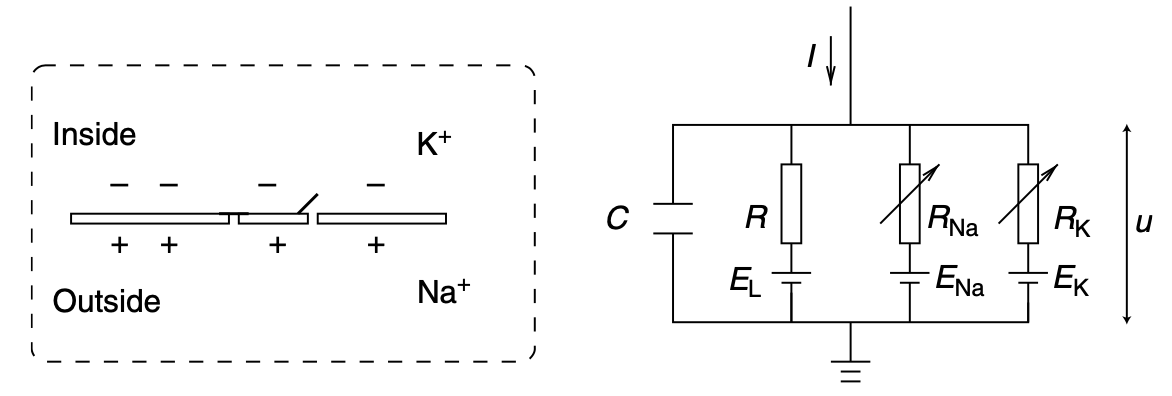
\includegraphics[width=13cm]{hodgkin_huxley_model}
	\caption{Schematic diagram of  Hodgkin-Huxley model}
	\label{fig:hodgkin_huxley_model}
\end{figure} 
  
\[
\sum_{k}I_k  = g_{Na}m^3h(u-E_{Na}) + g_{K}n^4(u-E_{K}) + g_{L}m^3h(u-E_{L})
\]

\subsubsection{Leaky integrate-and-fire model}


\subsection{Geometric deep learning theory}

\subsection{Reinforcement learning}

\subsection{Cognitive maps and hippocampus modelling}

\section{}

\paragraph{Problem statement} 
Let $\boldsymbol{x}$ be a sparse binary vector $\boldsymbol{x}\in\{0,1\}^n$ of length $n$. We observe signals  $\boldsymbol{x}$ coming from an unknown probability distribution $p(\boldsymbol{x})$. Our task is to build model $q(\boldsymbol{x})$ that matches $p(\boldsymbol{x})$ as closely as possible. We achieve this goal by modelling a latent one-hot vector $\boldsymbol{y}\in\{0,1\}^m$ of explanations and conditional probabilities $q(\boldsymbol{x}|y_j)$ corresponding to each explanation $y_j$ for $1\le j\le m$.
\[
q(\boldsymbol{x}) = \sum_{j=1}^m q(\boldsymbol{x}|y_j)p(y_j)
\]


\paragraph{Binary vector subsets and their overlap probabilities} 

We define cardinality $\lVert\boldsymbol{x}\rVert_1$ as the number of $1$ bits in a given binary vector $\boldsymbol{x}$.

The number of all sparse binary vectors $\boldsymbol{x}$ of length $n$ and cardinality $\lVert\boldsymbol{x}\rVert_1=b$ is
\[\binom{n}{b}\]
The $\ell_1$ norm induces a metric $\lVert\boldsymbol{x}-\boldsymbol{x}'\rVert_1$ on sparse binary vectors that measures how many bits differ in $\boldsymbol{x}$ and $\boldsymbol{x}'$. The inner product $\langle\boldsymbol{x},\boldsymbol{x}'\rangle$ measures number of overlapping $1$ bits. 
Given a specific $\boldsymbol{x}$, the number of all possible vectors $\boldsymbol{x}'$ that overlap with it in exactly $b$ bits is 
\[
\Omega(b)=|\{x':\langle\boldsymbol{x},\boldsymbol{x}'\rangle=b\}|=\binom{\lVert\boldsymbol{x}\rVert_1}{b}\binom{n-\lVert\boldsymbol{x}\rVert_1}{\lVert\boldsymbol{x}'\rVert_1-b}
\]
Therefore the probability that randomly chosen $\boldsymbol{x}'$ overlaps with $\boldsymbol{x}$ in at least $b$ bits is
\[p(\langle\boldsymbol{x},\boldsymbol{x}'\rangle\ge b )=\frac{\sum_{\dot{b}=b}^{\lVert\boldsymbol{x}'\rVert_1}\Omega(\dot{b})}{\binom{n}{\lVert\boldsymbol{x}\rVert_1}}\]
The probability of random $\boldsymbol{x}'$ being a subset of $\boldsymbol{x}$ is
\[p(\boldsymbol{x}'\subset\boldsymbol{x})=\frac{2^{\lVert\boldsymbol{x}\rVert_1}}{\binom{n}{\lVert\boldsymbol{x}\rVert_1}}\]
Both of those probabilities decrease factorially quickly with length $n$. For very sparse vectors, the chance of accidental overlap is almost zero. 

\paragraph{Formal definition of (first-order) ECC network}
Let us formally define ECC as a tuple $(Q,D_W,u,C,\boldsymbol{a})$. Matrix $Q\in \mathbb{R}^{n\times m}$ stores values of $q(x_i|y_j)$. Set $D_W$ specifies the domain of scalar values for some weight matrix $W\in D_W^{n \times m}$. Constant $u$ defines some norm $\ell_u$.  Vector $\boldsymbol{a}$ imposes length constraint on $\lVert W_j \rVert_u=a_j$ where $W_j\in D_W^n$ is the $j^{th}$ column of $W$. Set $C$ defines some partitioning (clustering) of input space $\boldsymbol{x}\in \{0,1\}^n$ into $m$ non-overlapping subsets $C(y_j) $.
Weights $W$ are defined as
\begin{gather*}
	W_j = \argmax_{W_j\in D_W^{n}} \mathbb{E}_p(\boldsymbol{x}W_j|y_j)\text{ where } \lVert W_j \rVert_u=a_j \\
	\mathbb{E}_p(\boldsymbol{x}W_j|y_j) = \sum_{\boldsymbol{x}\in C(y_j)}\boldsymbol{x}W_jp(\boldsymbol{x}|y_j) \\ 
	p(\boldsymbol{x}|y_j) = \frac{p(\boldsymbol{x},y_j)}{p(y_j)} \\
	p(y_j) =  \sum_{\boldsymbol{x}\in \{0,1\}^n}p(\boldsymbol{x},y_j)
\end{gather*}
The clustering assigns every $\boldsymbol{x}$ to its respective $C(y_j)$. Therefore 
\[
p(\boldsymbol{x},y_j) = \begin{cases}
	p(\boldsymbol{x}) & \boldsymbol{x} \in C(y_j) \\
	0 & \boldsymbol{x} \notin C(y_j)
\end{cases}
\]
As a result we can simplify $p(\boldsymbol{x}|y_j)$ and $p(y_j)$ to
\begin{gather*}
p(\boldsymbol{x}|y_j) = \frac{p(\boldsymbol{x})}{p(y_j)}, \text{ where  }\boldsymbol{x} \in C(y_j)\\
p(y_j) =  \sum_{\boldsymbol{x}\in C(y_j)}p(\boldsymbol{x})
\end{gather*}
The distribution $p(\boldsymbol{x}|y_j)$ is not known and the exact $W_j$ cannot be computed. Instead, ECC network attempts to approximate $p$ using $q$ 
\[
p(\boldsymbol{x}|y_j) \approx q(\boldsymbol{x}|y_j)
\]
First-order ECC networks model the distribution $q$ using the matrix $Q$. 
Under the assumption that all bits $q(x_i|y_j)$ are mutually independent random variables we obtain
\[
q(\boldsymbol{x}|y_j) = \prod_{i=1}^n q(x_i|y_j)
\]
In the case of $\ell_1$ and $\ell_2$, it is possible to compute $W_j$ using only  $Q$ and without having to model $q(\boldsymbol{x}|y_j)$ directly (convergence proofs work even without assuming mutual independence of $x_i$ bits).

\paragraph{Learning is achieved by maximising $q(\boldsymbol{x}|y_k)$}
The probability $q(\boldsymbol{x})$ is modelled as
\[
q(\boldsymbol{x}) = \sum_{j=1}^{m} q(\boldsymbol{x}|y_j)p(y_j)
\]
We can find good approximation $q(\boldsymbol{x})\approx p(\boldsymbol{x})$, by ensuring that $q(\boldsymbol{x}|y_j)\approx p(\boldsymbol{x}|y_j)$. 
\begin{gather*}
	q(\boldsymbol{x}) \approx p(\boldsymbol{x}) \\
	\sum_{j=1}^{m} q(\boldsymbol{x}|y_j)p(y_j) \approx \sum_{j=1}^{m} p(\boldsymbol{x}|y_j)p(y_j) \\
	\sum_{j=1}^{m} q(\boldsymbol{x}|y_j)p(y_j)  \approx p(\boldsymbol{x}|y_k)p(y_k) \text{ where }\boldsymbol{x}\in C(y_k)
\end{gather*}
By subtracting $p(\boldsymbol{x}|y_k)p(y_k)$ from both sides, it implies that $ q(\boldsymbol{x}|y_j)$ should be minimised for all $j$ such that $\boldsymbol{x}\notin C(y_j)$
\[
	\sum_{j\ne k} q(\boldsymbol{x}|y_j)p(y_j) \approx 0 
\]
Minimisation of $q(\boldsymbol{x}|y_k)$ for $\boldsymbol{x}\notin C(y_k)$ is equivalent to maximization of $\sum_{\boldsymbol{x}\in C(y_k)}q(\boldsymbol{x}|y_k)$ because probabilities sum up to $1$. 
\[
\sum_{\boldsymbol{x}\in\{0,1\}^n} \sum_{j=1}^{m} q(\boldsymbol{x}|y_j)p(y_j) = 1
\]
If $\sum_{\boldsymbol{x}\notin C(y_j)} q(\boldsymbol{x}|y_j)$ decreases across all $y_j$ and $p(y_j)$ stay constant then the following sum decreases
\[
\sum_{j} \sum_{\boldsymbol{x}\notin C(y_j)} q(\boldsymbol{x}|y_j) p(y_j) = \sum_{\boldsymbol{x}} \sum_{j\ne k}  q(\boldsymbol{x}|y_j) p(y_j) \text{ where }\boldsymbol{x}\in C(y_k)
\]
Therefore it can be seen that maximization of $\sum_{\boldsymbol{x}\in C(y_k)}q(\boldsymbol{x}|y_k)$ will push $q$ closer to $p$. This observation is fortunate, because Hebbian learning rules strengthen connections to those $\boldsymbol{x}$ that cause $y_j$ to fire.

\paragraph{Clustering problem measured with overlap}
We can measure quality of cluster $C(y_j)$ as the expected overlap $\langle \boldsymbol{x}, \boldsymbol{x}'\rangle$ (number of $1$ bits in common) of two binary vectors  randomly drawn from the distribution $p(\boldsymbol{x}|y_j)$.
\[
\mathbb{E}_p(\langle \boldsymbol{x}, \boldsymbol{x}'\rangle|y_j) = \sum_{\boldsymbol{x},\boldsymbol{x}'\in C(y_j)} \langle \boldsymbol{x}, \boldsymbol{x}'\rangle p(\boldsymbol{x}|y_j)p(\boldsymbol{x}'|y_j)
\]
The expectation of any two vectors overlapping in a specific bit $x_i$ is given by
\begin{gather*}
p(x_i|y_j) = \sum_{\substack{\boldsymbol{x}\in C(y_j)\\x_i=1}} p(\boldsymbol{x}|y_j)	= \sum_{\boldsymbol{x}\in C(y_j)} x_i p(\boldsymbol{x}|y_j)	= \mathbb{E}(x_i|y_j)\\
\mathbb{E}_p(x_i x_i' | y_j) = \sum_{\boldsymbol{x},\boldsymbol{x}'\in C(y_j)}  x_i x_i' p(\boldsymbol{x}|y_j)p(\boldsymbol{x}'|y_j) = 	\sum_{\substack{\boldsymbol{x},\boldsymbol{x}'\in C(y_j) \\ x_i=x_i'=1}} p(\boldsymbol{x}|y_j)p(\boldsymbol{x}'|y_j) = \\
= \sum_{\substack{\boldsymbol{x}\in C(y_j) \\ x_i=1}} p(\boldsymbol{x}|y_j) \sum_{\substack{\boldsymbol{x}'\in C(y_j) \\ x_i'=1}} p(\boldsymbol{x}'|y_j) = 
\sum_{\substack{\boldsymbol{x}\in C(y_j) \\ x_i=1}} p(\boldsymbol{x}|y_j) \mathbb{E}(x_i'|y_j)= \\
= \mathbb{E}(x_i'|y_j) \sum_{\substack{\boldsymbol{x}\in C(y_j) \\ x_i=1}} p(\boldsymbol{x}|y_j) = \mathbb{E}(x_i'|y_j) \mathbb{E}(x_i|y_j) = \mathbb{E}(x_i|y_j)^2
\end{gather*}
Therefore the expected value of overlap can be rewritten as  
\begin{gather*}
\mathbb{E}_p(\langle \boldsymbol{x}, \boldsymbol{x}'\rangle|y_j) =  \sum_{\boldsymbol{x},\boldsymbol{x}'\in C(y_j)} \big(\sum_{i=1}^n x_i x_i'\big)  p(\boldsymbol{x}|y_j)p(\boldsymbol{x}'|y_j) = \\
= \sum_{i=1}^n \sum_{\boldsymbol{x},\boldsymbol{x}'\in C(y_j)}  x_i x_i'  p(\boldsymbol{x}|y_j)p(\boldsymbol{x}'|y_j) = \sum_{i=1}^n \mathbb{E}(x_i|y_j)^2 = \lVert \mathbb{E}(\boldsymbol{x}|y_j) \rVert_2^2
\end{gather*}

\paragraph{Expected overlap and $Q$ matrix} 
The expected overlap can be expressed in terms of the matrix $Q$
\[
\mathbb{E}(\langle \boldsymbol{x}, \boldsymbol{x}'\rangle|y_j) = \lVert \mathbb{E}(\boldsymbol{x}|y_j) \rVert_2^2 =  \lVert Q_j \rVert_2^2
\]
or as a dot product $\boldsymbol{x}Q$
\begin{gather*}
	\mathbb{E}_p(x_i x_i' | y_j) = 
	\sum_{\substack{\boldsymbol{x}\in C(y_j) \\ x_i=1}} p(\boldsymbol{x}|y_j) \mathbb{E}(x_i'|y_j)= \mathbb{E}_p\big(x_i \mathbb{E}(x_i'|y_j) \big| y_j\big) = \mathbb{E}_p\big(x_i p(x_i|y_j) \big| y_j'\big)\\
	\mathbb{E}_q(\langle \boldsymbol{x}, \boldsymbol{x}'\rangle|y_j) = \mathbb{E}(\boldsymbol{x} Q_j | y_j)
\end{gather*}

\paragraph{Zero-order ECC networks}
In the first-order ECC network, we defined weights by finding $W_j$ that maximise product $\boldsymbol{x}W_j$
\begin{gather*}
	W_j = \argmax_{W_j\in D_W^{n}} \mathbb{E}_p(\boldsymbol{x}W_j|y_j)\text{ where } \lVert W_j \rVert_u=a_j
\end{gather*}
In zero-order ECC network we assume that $Q=W$. Then maximisation of $\boldsymbol{x}W$ is synonymous with maximisation of both $\boldsymbol{x}Q$ and $\mathbb{E}(\langle \boldsymbol{x}, \boldsymbol{x}'\rangle|y_j) $. 
The implication holds trivially by equality
\[
\boldsymbol{x}W_j \le \boldsymbol{x}W_h  \implies  \boldsymbol{x}Q_j \le \boldsymbol{x}Q_h 
\]
\paragraph{Optimal clustering maximises $p(\boldsymbol{x}|y_k)$} 
The effectiveness of neurons depends on their ability to maximise $q(\boldsymbol{x}|y_j)$ for all inputs that belong to a given cluster $\boldsymbol{x}\in C(y_j)$ and minimise $q(\boldsymbol{x}|y_j)$ for those that don't  $\boldsymbol{x}\notin C(y_k)$. In an ideal case $q(\boldsymbol{x}|y_j)$ would be $0$ for all $\boldsymbol{x}\notin C(y_j)$. 

The $Q$ matrix is not capable of fitting every distribution $q(\boldsymbol{x}|y_k)$.
If we assume that
\[
C(y_j) = \{\boldsymbol{x}:j=\argmax \boldsymbol{x}W\}
\]
then the network could use $W$ matrix to optimally cluster $\boldsymbol{x}$ in a way that makes the task of fitting $q(\boldsymbol{x}|y_j)$ easier for $Q$. If we can show
\[
\boldsymbol{x}W_j \le \boldsymbol{x}W_h  \implies  \boldsymbol{x}Q_j \le \boldsymbol{x}Q_h 
\]
then it would imply that maximisation of $\boldsymbol{x}W_j$ leads to higher overlap
$\mathbb{E}(\langle \boldsymbol{x}, \boldsymbol{x}'\rangle|y_j) $. If most inputs $\boldsymbol{x}\in C(y_j)$ share many bits in common, then $Q_j$ can better fit $p(\boldsymbol{x}|y_j)$ by assigning higher probabilities only to those highly frequent bits and near-zero everywhere else. This leads to agreement between $p$ and $q$. 



\paragraph{Expected value $\mathbb{E}_{p}(\boldsymbol{x}|y_j)$ maximises $\boldsymbol{x}W_j$ under $\ell_2$ norm} 

We wish to maximise the expected value of $\boldsymbol{x}W_j$
\[
\mathbb{E}_{p}(\boldsymbol{x}W_j|y_j)=\sum_{\boldsymbol{x}\in C(y_j)} \boldsymbol{x} W_j p(\boldsymbol{x}|y_j)
\]
 under the constraint $\lVert W_j \rVert_2 = a_j$ for some constant $a_j$.  To find the optimal $W_j$, we can use the method of Lagrange multipliers
\[
L(W_j,\lambda) = \sum_{\boldsymbol{x}\in C(y_j)} \boldsymbol{x} W_j p(\boldsymbol{x}|y_j) + \lambda(1- W_j^{T}W_j )
\]
The term $\lambda(1- W_j^{T}W_j)$ will be $0$ only when $W_j$ is a unit vector.
We can take the derivatives 
\begin{gather*}
	\frac{d L}{d w_{ij}} = \sum_{\boldsymbol{x}\in C(y_j)} x_i p(\boldsymbol{x}|y_j) - 2\lambda w_{ij} \\
	\frac{d L}{d \lambda} = 1 - W_j^{T}W_j
\end{gather*}
and solve for $\frac{d L}{d w_{ij}}=0$
\[
W_j = \frac{1}{2\lambda }\sum_{\boldsymbol{x}\in C(y_j)} \boldsymbol{x} p(\boldsymbol{x}|y_j)  = \frac{1}{2\lambda } \mathbb{E}_{p}(\boldsymbol{x}|y_j)
\]
By taking the second derivative we can show that this is indeed a local maximum.
The problem is convex (there is only one extremum), because all observations are binary vectors (Frechet mean on $S^{n-1}$ unit sphere is unique if all points lie on the same hemisphere) and the expected value $\mathbb{E}_{p}(\boldsymbol{x}|y_j)$ will never be a zero vector.

It should be noted that such expected value will be skewed more towards the $\boldsymbol{x}$ with greater cardinality. To avoid any biases, it is necessary to normalise the vectors 
\[
\mathbb{E}_{p}\big(\frac{\boldsymbol{x}}{\lVert \boldsymbol{x} \rVert_2}W_j|y_j \big)= \sum_{\boldsymbol{x}\in C(y_j)} \frac{\boldsymbol{x}}{\lVert \boldsymbol{x} \rVert_2} W_j p(\boldsymbol{x}|y_j)
\]


\paragraph{One-hot vector maximizes $\boldsymbol{x}W$ under $\ell_1$ norm}
We wish to maximise the expected value of $\boldsymbol{x}W_j$ 
\[
\mathbb{E}_{p}(\boldsymbol{x}W_j|y_j)=\sum_{\boldsymbol{x}\in C(y_j)} \boldsymbol{x} W_j p(\boldsymbol{x}|y_j) \text{ where } \lVert W_j \rVert_1=1
\]
sampled according to some distribution $p(\boldsymbol{x}|y_j)$ from a given set $\boldsymbol{x}\in C(y_j)$.  The sum can be rewritten as
\[
\sum_{\boldsymbol{x}\in C(y_j)} \boldsymbol{x} W_j p(\boldsymbol{x}|y_j) = \mathbb{E}_{p}(\boldsymbol{x} W_j|y_j) = \mathbb{E}_{p}(\boldsymbol{x}|y_j)W_j
\]
because $\mathbb{E}$ is a linear operator. The value of $\mathbb{E}_{p}(\boldsymbol{x}|y_j)$ is some real vector $\mathbb{R}^n$.  It can be observed that $\mathbb{E}_{p}(\boldsymbol{x}|y_j)W_j$ is maximised when $W_j$ is a one-hot vector with $w_{ij}=1$ for such $i$ where $p(x_i|y_j)$ is maximal. 

\paragraph{Generalized $a_j$-hot vector maximizes $\boldsymbol{x}W$ under $\ell_1$ norm}
The result above can be generalised for $\lVert W_j \rVert_1 = a_j$ where $a_j$ is any positive constant, not just $1$. When $a_j=1$, then we have a guarantee that $w_{ij}\le 1$ for all $i$. Hence our original definition of $W_j$ was a real vector $W_j\in \mathbb{R}^n$, but implicitly it was only $W_j\in [0,1]^n$. 

When $a_j\ne 1$, then we must be explicit and state exactly the allowed range of values for $w_{ij}$. Let us consider a scenario where $a_j\in\mathbb{N}^+$ and $W_j\in [0,1]^n$, then the value of $W_j$ that maximizes $\mathbb{E}_{p}(\boldsymbol{x}|y_j)W_j$ is an $a_j$-hot vector with $w_{ij}=1$ for all $i$ such that $p(x_i|y_j)$ is among the top $a_j$ highest probabilities. 

If $a_j\in\mathbb{R}^+$ and $W_j\in [0,1]^n$ then we can maximise $\mathbb{E}_{p}(\boldsymbol{x}|y_j)W_j$ using similar strategy. First we find the $\lfloor a_j \rfloor$ highest values $p(x_i|y_j)$ and assign $w_{ij}=1$ for all those $i$. Lastly we find the $\lfloor a_j \rfloor+1$ highest value of $p(x_i|y_j)$ and assign the remaining fractional value to $w_{ij}=a_j - \lfloor a_j \rfloor$. 

For example let 
\[
\mathbb{E}_{p}(\boldsymbol{x}|y_j) = [0.2,0.3,0.8,0.7,0.4]
\]
If $a_j=3$ then maximal $\mathbb{E}_{p}(\boldsymbol{x}|y_j)W_j$ is obtained for 
\[
W_j=[0,0,1,1,1]
\]
If $a_j=2.3$ then maximum is at
\[
W_j=[0,0,1,1,0.3]
\]

\paragraph{Generalised proof of k-means convergence for first-order networks}
Start with some arbitrary $C^{(0)}$ at time step $t=0$. Given $C^{(t)}$ compute $Q^{(t)}$
\[
Q^{(t)}_j = \mathbb{E}_p(\boldsymbol{x}|y_j)
\]
Given $C^{(t)}$ and $Q^{(t)}$ compute weights $W^{(t)}$
\begin{gather*}
	W_j^{(t)} = \argmax_{W_j\in D_W^{n}} \mathbb{E}_p(\boldsymbol{x}W_j|y_j)\text{ where } \lVert W_j \rVert_u=a_j
\end{gather*}
Given $W^{(t)}$ compute new clusters $C^{(t)}$
\[
C^{(t+1)}(y_j) = \{\boldsymbol{x} : j=\argmax(\boldsymbol{x}W^{(t)})\}
\]
To show that convergence is guaranteed let us define a fitness function
\[
\mathcal{L}^{(t)} = \sum_{j=1}^m \sum_{\boldsymbol{x}\in C^{(t)}(y_j)} \boldsymbol{x} W_j^{(t)} p(\boldsymbol{x})
\] 
This function is bounded from above by some constant that depends on $\boldsymbol{a}$. We can show that it is monotonously non-decreasing. The proof is done in two steps. First we show inequality when $W_j^{(t)}$  is replaced by $W_j^{(t+1)}$
\[\mathcal{L}^{(t)}= \sum_{j=1}^m \sum_{\boldsymbol{x}\in C^{(t)}(y_j)} \boldsymbol{x} W_j^{(t)} p(\boldsymbol{x}) \le \sum_{j=1}^m \sum_{\boldsymbol{x}\in C^{(t)}(y_j)} \boldsymbol{x}W_j^{(t+1)} p(\boldsymbol{x})\] 
Second we show monotonicity when $C^{(t)}$ is updated to $C^{(t+1)}$
\[\sum_{j=1}^m \sum_{\boldsymbol{x}\in C^{(t)}(y_j)} \boldsymbol{x} W_j^{(t+1)} p(\boldsymbol{x}) \le \sum_{j=1}^m \sum_{\boldsymbol{x}\in C^{(t+1)}(y_j)} \boldsymbol{x} W_j^{(t+1)} p(\boldsymbol{x})=\mathcal{L}^{(t+1)}\] 
The first inequality holds because it can be rewritten as
\[\sum_{j=1}^m p(y_j) \mathbb{E}(\boldsymbol{x} W_j^{(t)}|y_j)  \le \sum_{j=1}^m  p(y_j)  \mathbb{E}(\boldsymbol{x}W_j^{(t+1)}|y_j)\] 
and we know that $W_j^{(t+1)}$ maximizes $\mathbb{E}(\boldsymbol{x}W_j^{(t+1)})$.
The second inequality holds, because any two clusters $C^{(t)}(y_j)$ and  $C^{(t+1)}(y_j)$ will differ only when there exists some $\boldsymbol{x}\in C^{(t)}(y_j)$ such that there is some other $y_h$ for which $\boldsymbol{x}W_h \ge \boldsymbol{x} W_j$. This implies that the total sum over all clusters cannot decrease.

\paragraph{Convergence is not guaranteed for zero-order networks}
The k-means procedure for zero-order networks is almost identical as above except that $W^{(t)}=Q^{(t)}$. The loss function becomes
\begin{gather*}
\mathcal{L}^{(t)} = \sum_{j=1}^m \sum_{\boldsymbol{x}\in C^{(t)}(y_j)} \boldsymbol{x} Q_j^{(t)} p(\boldsymbol{x}) = \sum_{j=1}^m p(y_j) \mathbb{E}(\boldsymbol{x} Q_j^{(t)}|y_j) = \\ 
= \sum_{j=1}^m p(y_j) \mathbb{E}(\langle \boldsymbol{x},\boldsymbol{x}' \rangle |y_j) 	 = \mathbb{E}(\langle \boldsymbol{x},\boldsymbol{x}' \rangle)
\end{gather*}
The previous proof no longer applies, because $Q_j$ does not maximise $\mathbb{E}(\boldsymbol{x}W_j|y_j)$. Empirical benchmarks showed that the fitness function increases and converges but doesn't do it monotonously. 
\paragraph{Convergence of $Q$ in online-learning}
In the proofs based on k-means algorithm we were allowed to compute $Q$ exactly. 
\[
Q_j = \sum_{\boldsymbol{x}\in C(y_j)}\boldsymbol{x}p(\boldsymbol{x}|y_j)
\]
If we do not have access to $p$, we could use empirical distribution $\bar{p}$, given to us in form of some observed sample (dataset). In the case of online-learning our algorithm receives an infinite stream of samples that cannot be stored or replayed. We can still approximate $Q$ with the following algorithm
\begin{lstlisting}
$Q_j$ = random_initialization()
for $\boldsymbol{x}$ sampled from $p(\boldsymbol{x}|y_j)$:
    $Q_j$ = $(1-\epsilon)Q_j + \epsilon \boldsymbol{x}$ 
\end{lstlisting}
This is a moving-average approximation of $p(x_i|y_j)$, which converges due to central limit theorem (CLT). To prove it, suppose $\boldsymbol{x}_1,\boldsymbol{x}_2,...,\boldsymbol{x}_t$ is a sample and $\bar{\boldsymbol{x}}$ is it's mean. Then after observing new $\boldsymbol{x}_{t+1}$, the updated mean is $\frac{t\bar{\boldsymbol{x}} + \boldsymbol{x}_{t+1} }{t+1}$. If we put $\epsilon=\frac{1}{\text{t+1}}$, then CLT states that $\bar{\boldsymbol{x}}$ approaches $\mathbb{E}(\boldsymbol{x}|y_j)$ as $t$ goes to infinity. As $x_i$ is a binary random variable, it implies that $\mathbb{E}(x_i|y_j)=p(x_i|y_j)$. Hence if we choose small $\epsilon$, then $Q$ will approximate $p$ with greater precision.

There also exists an alternative algorithm that can approximates $p(i|y_j)$ instead of $p(x_i|y_j)$. It is defined as
\begin{gather*}
	q(i|y_j) = \frac{q(x_i=1|y_j)}{\sum_{ï=0}^n{q(x_{ï}=1|y_j)}} \\
	\sum_{i=1}^n q(x_{i}|y_j) =  \lVert \mathbb{E}_q( \boldsymbol{x}|y_j) \rVert_1 = \mathbb{E}_q(\lVert \boldsymbol{x} \rVert_1|y_j) \\
	q(x_i|y_j) = \begin{cases}
		q(i|y_j)\mathbb{E}_q(\lVert \boldsymbol{x} \rVert_1|y_j)&\text{if }x_i=1 \\
		1-q(i|y_j)\mathbb{E}_q(\lVert \boldsymbol{x} \rVert_1|y_j)&\text{if }x_i=0 
	\end{cases}
\end{gather*}
The algorithm computes a moving average of vectors, rather than individual scalars
\begin{lstlisting}
$Q_j$ = random_initialization()
for $\boldsymbol{x}$ sampled from $p(\boldsymbol{x}|y_j)$:
    $Q_j$ = $Q_j + \epsilon \boldsymbol{x}$ 
    $Q_j$ = $Q_j$/$\lVert Q_j \rVert_1$
\end{lstlisting}

\paragraph{Higher-order networks}

The distribution $q(\boldsymbol{x})$ is modelled as a sum
\[
q(\boldsymbol{x}) = \sum_{j=1}^{m}q(\boldsymbol{x}|y_j)p(y_j) 
\]
Such factorization is motivated by the assumption that the external world has many latent causes $y_j$, and every one of them produces noisy observations $x_i$. The real world could potentially be approximated using trillions of latent causes, each one corresponding to some state of the world and objects in it. 

Many of the latent causes will produce similar or nearly identical observations. Could we exploit those similarities and compress our model, so that $m$ is as small as possible? 

One way to reduce the number of $y$'s is by adding two (or more) of them as follows
\[
q(\boldsymbol{x}|y_1) p(y_1)+q(\boldsymbol{x}|y_2) p(y_2) = 
q(\boldsymbol{x}|y_1\text{ or }y_2) (p(y_1)+p(y_2))
\]
but storing $q(\boldsymbol{x}|y_1\text{ or }y_2)$ directly is impossible, because $Q$ can only be used to represent mutually independent bits $x_i$. 
\[
\frac{q(\boldsymbol{x}|y_1;Q_1) p(y_1)+q(\boldsymbol{x}|y_2;Q_2) p(y_2)}{p(y_1)+p(y_2)} \ne 
q\big(\boldsymbol{x}|y_1\text{ or }y_2;\frac{Q_1p(y_1) +Q_2p(y_2)}{p(y_1)+p(y_2)}\big) 
\]
The first-order ECC networks modelled the conditional distribution $q(\boldsymbol{x}|y_1)$ as
\[
q(\boldsymbol{x}|y_1) = \prod_{i=1}^{n}q(x_i|y_1)
\]
Second-order networks are allowed to model distribution $q(\boldsymbol{x}|y_1\text{ or }y_2)$. 
\[
q(\boldsymbol{x}|y_1\text{ or }y_2) = \prod_{i=1}^{n}q(x_i|y_1) + \prod_{i=1}^{n}q(x_i|y_2)
\]
In this case, the network has a single neuron unit ``$y_1\text{ or }y_2$'' that has two ``dendritic segments'' $y_1$ and $y_2$. The neuron will activate if any of its dendrites is excited. Analogically, third-order ECC have the capacity to model $q(\boldsymbol{x}|y_1\text{ or }y_2\text{ or }y_3)$. 
\[
q(\boldsymbol{x}|y_1\text{ or }y_2\text{ or }y_3) = \prod_{i=1}^{n}q(x_i|y_1) + \prod_{i=1}^{n}q(x_i|y_2) + \prod_{i=1}^{n}q(x_i|y_3)
\]
Higher-order networks are allowed to ``factor out'' certain common bits. For example suppose $n=2$, then we could model $y_*$ as a mix of $y_1$, $y_2$ and $y_3$ with additional assumption of to equality $q(x_1|y_1)=q(x_1|y_2)$
\[
q(\boldsymbol{x}|y_*) = q(x_1|y_1)\big(q(x_2|y_1) +q(x_2|y_1)\big) + q(x_1|y_3)q(x_2|y_3)
\]
More generally, higher-order network is the union of $1,2,3...$-order networks with equality constraints of the form $q(x_{i_1}|y_{j_1})=q(x_{i_2}|y_{j_2})$. Factoring out common bits leads to equations with a tree-like nested structure of brackets.
This may closely resemble dendritic trees of biological neurons.

\paragraph{Top k-winners take all}
In the original definition, clustering $C$ partitions the inputs space into mutually disjoint subsets. We can relax this assumption and allow for a single $\boldsymbol{x}$ to be included in $k$ different clusters $C(y_{j_1}),C(y_{j_2}),...C(y_{j_k})$.
We define conditional probability $q(\boldsymbol{x}|\boldsymbol{y})$ as
\[
q(\boldsymbol{x}|\boldsymbol{y}) = \prod_{y_j \in \boldsymbol{y}} q(\boldsymbol{x}|y_j)
\]
The cardinality $\lVert \boldsymbol{y} \rVert_1$ corresponds to the number of clusters $k$. Note that if $k=1$, then $q(\boldsymbol{x}|\boldsymbol{y})=q(\boldsymbol{x}|y_j)$, hence the new definition is a generalisation of first-order networks.
We assume that $q(\boldsymbol{x}|y_j)$
The probability $q(\boldsymbol{x})$ is defined as
\[
q(\boldsymbol{x}) = \sum_{\boldsymbol{y}} q(\boldsymbol{x}|\boldsymbol{y})
\]


 
\bibliographystyle{BibTeXtran}   % (uses file "BibTeXtran.bst")
\bibliography{BibTeXrefs}    







\end{document}
